\documentclass[12pt]{article}


% ----------------- PAQUETES -----------------
\usepackage[utf8]{inputenc}
\usepackage[spanish]{babel}
\usepackage[margin = 2.54cm]{geometry}
\usepackage{graphicx}
\usepackage{enumitem}
\usepackage{parskip}
\usepackage{bm}
\usepackage[x11names,table]{xcolor}
\usepackage{amsmath}



% ----------------- CONFIGURACIONES -----------------
% ----------------- UTILIDADES PARA DAR UN MEJOR FORMATO DE DOCUMENTO -----------------  


\definecolor{azul}{rgb}{0.0039, 0.3098, 0.6196}


% Formato para el indice general ...........
\makeatletter
    \renewcommand{\@dotsep}{1.5}
    \renewcommand{\l@section}{\@dottedtocline{1}{1.5em}{2.3em}}
    \renewcommand{\l@subsection}{\@dottedtocline{2}{3.8em}{3.2em}}
    \renewcommand{\l@subsubsection}{\@dottedtocline{3}{7.0em}{4.1em}}
\makeatother

% --------- COMANDOS PERSONALIZADOS PARA LA PORTADA DE LAS TAREAS, TRABAJOS Y PROYECTOS ---------

\newcommand{\rutaLogo}[1]{\newcommand{\RutaLogo}{#1}}
\newcommand{\tema}[1]{\newcommand{\Tema}{#1}}
\newcommand{\etiquetaAutores}[1]{\newcommand{\EtiquetaAutores}{#1}}
\newcommand{\alumno}[1]{\newcommand{\Alumno}{#1}}
\newcommand{\materia}[1]{\newcommand{\Materia}{#1}}
\newcommand{\docente}[1]{\newcommand{\Docente}{#1}}
\newcommand{\ciclo}[1]{\newcommand{\Ciclo}{#1}}
\newcommand{\fecha}[1]{\newcommand{\Fecha}{#1}}
\newcommand{\periodo}[1]{\newcommand{\Periodo}{#1}}

\definecolor{celeste}{HTML}{94E4F1}


% ----------------- PORTADA -----------------
\rutaLogo{../../../docs/img/logo-ista.png}
\tema{\\ \vspace{0.8cm} Taller de ejercicios - Límites \\ \vspace{1.5cm}}
\etiquetaAutores{Alumno: }
\alumno{Eduardo Mendieta \vspace{0.8cm}}
\materia{Matemática \vspace{0.8cm}}
\docente{Lcda. Vilma Duchi, Mgtr. \vspace{0.8cm}}
\ciclo{Primer ciclo \vspace{0.8cm}}
\fecha{05/08/2024 \vspace{0.8cm}}
\periodo{Abril 2024 - Agosto 2024}


\begin{document}
    \begin{titlepage}

    \centering

    \includegraphics[width=0.11\textwidth]{\RutaLogo} 

    \vspace{0.3cm}
    \textcolor{azul}{\Large \textbf{Instituto Superior Universitario Tecnológico del Azuay \\}}
    \vspace{0.3cm}
    \textcolor{azul}{\Large \textbf{Tecnología Superior en Big Data}}
    
    % 1. ---------------- TEMA -------------------------
    
    {\Large\textbf{\Tema}}
    
    % 2. ---------------- AUTOR(ES) -------------------------
    \textcolor{azul}{\large \textbf{\EtiquetaAutores} \\}
    \vspace{0.3cm}
    {\large \Alumno}

    % 3. ---------------- MATERIA -------------------------
    \textcolor{azul}{\large \textbf{Materia:} \\}
    \vspace{0.3cm}
    {\large \Materia}


    % 3. ---------------- DOCENTE -------------------------
    \textcolor{azul}{\large \textbf{Docente:} \\}
    \vspace{0.3cm}
    {\large \Docente}


    % 3. ---------------- Ciclo -------------------------
    \textcolor{azul}{\large \textbf{Ciclo:} \\}
    \vspace{0.3cm}
    {\large \Ciclo}


    % 3. ---------------- FECHA -------------------------
    \textcolor{azul}{\large \textbf{Fecha:} \\}
    \vspace{0.3cm}
    {\large \Fecha}

    % 3. ---------------- PERIODO -------------------------
    \textcolor{azul}{\large \textbf{Periodo Académico:} \\}
    \vspace{0.3cm}
    {\large \Periodo}
 
\end{titlepage}


    \section*{\centering Taller de ejercicios - Límites}
        \textbf{Resolver los siguientes ejercicios:} \vspace{1cm} \hrule

        \begin{enumerate}[label=\textbf{\arabic*.}]
            % EJERCICIO 1: ---------------------------------------------------
            \item \textbf{Estime el valor del límite haciendo una tabla de valores, compruebe su trabajo con una gráfica:}
                \begin{enumerate}[label=\textbf{\arabic*)}] 
                    \item \[\bm{\lim_{x \to 5} \frac{x ^2 - 25}{x - 5}} \approx 10 \] 
                     
                        \begin{itemize}
                            \item $\frac{4.9^2 - 25}{4.9 - 5} = 9.9$ \hspace{1cm} $\frac{4.99^2 - 25}{4.99 - 5} = 9.99$ \hspace{1cm} $\frac{4.999^2 - 25}{4.999 - 5} = 9.999$
                            \item $\frac{5.001^2 - 25}{5.001 - 5} = 10.001$ \hspace{1cm} $\frac{5.01^2 - 25}{5.01 - 5} = 10.01 $ \hspace{1cm} $\frac{5.1^2 - 25}{5.1 - 5} = 10.1 $
                        \end{itemize}

                        \begin{table}[h]
                            \centering
                            \begin{tabular}{|>{\columncolor{celeste}}l|l|l|l|l|l|l|l|l|l|l|l|}
                                \hline
                                $\bm{x}$    & 4.9 & 4.99 & 4.999  & \textbf{5} & 5.001 & 5.01 & 5.1 \\
                                \hline
                                $\bm{f(x)}$ & 9.9 & 9.99 & 9.999  & \textit{10} & 10.001 & 10.01 & 10.1 \\
                                \hline
                            \end{tabular}
                        \end{table}

                        \begin{figure}[h!]
                            \centering
                            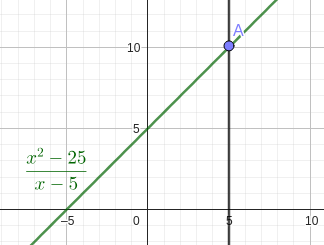
\includegraphics[width=0.4\textwidth]{img/t1-ej1-1.png}
                        \end{figure}



                    \item \[\bm{\lim_{x \to 3} \frac{x ^2 - x - 6}{x - 3}} \approx 5\]
                        
                        \begin{itemize}
                            \item $\frac{2.9^2 - 2.9 - 6}{2.9 - 3} = 4.9 $ \hspace{1cm} $\frac{2.99^2 - 2.99 - 6}{2.99 - 3} = 4.99 $ \hspace{1cm} $\frac{2.999^2 - 2.999 - 6}{2.999 - 3} = 4.999 $
                            \item $\frac{3.001^2 - 3.001 - 6}{3.001 - 3} = 5.001 $ \hspace{1cm} $\frac{3.01^2 - 3.01 - 6}{3.01 - 3} = 5.01 $ \hspace{1cm} $\frac{3.1^2 - 3.1 - 6}{3.1 - 3} = 5.1 $
                        \end{itemize}

                        \begin{table}[h]
                            \centering
                            \begin{tabular}{|>{\columncolor{celeste}}l|l|l|l|l|l|l|l|l|l|l|l|}
                                \hline
                                $\bm{x}$    & 2.9 & 2.99 & 2.999  & \textbf{3} & 3.001 & 3.01 & 3.1 \\
                                \hline
                                $\bm{f(x)}$ & 4.9 & 4.99 & 4.999  & \textit{5} & 5.001 & 5.01 & 5.1 \\
                                \hline
                            \end{tabular}
                        \end{table}

                        \newpage
                        \begin{figure}[h!]
                            \centering
                            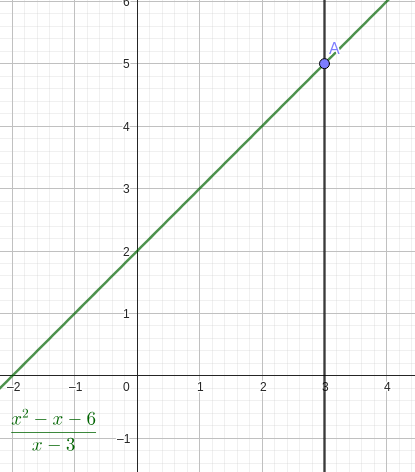
\includegraphics[width=0.4\textwidth]{img/t1-ej1-2.png}
                        \end{figure}

                \end{enumerate}


            % EJERCICIO 2: ---------------------------------------------------
            \vspace{1cm}\hrule
            \item \textbf{Complete la tabla de valores (a cinco lugares decimales), y use la tabla para estimar el valor del límite:}
                \begin{enumerate}[label=\textbf{\arabic*)}] 
                    \item \[\bm{\lim_{x \to 4} \frac{\sqrt{x} - 2}{x - 4}} \approx 0.25 \]
                        
                        \begin{itemize}
                            \item $\frac{\sqrt{3.9} - 2}{3.9 - 4} = 0.252$ \hspace{1cm} $\frac{\sqrt{3.99} - 2}{3.99 - 4} = 0.25$ \hspace{1cm} $\frac{\sqrt{3.999} - 2}{3.999 - 4} = 0.25$ \vspace{0.2cm} \\ $\frac{\sqrt{3.9999} - 2}{3.9999 - 4} = 0.25$ \hspace{1cm} $\frac{\sqrt{3.99999} - 2}{3.99999 - 4} = 0.25$
                            \item $\frac{\sqrt{4.00001} - 2}{4.00001 - 4} = 0.25$ \hspace{1cm} $\frac{\sqrt{4.0001} - 2}{4.0001 - 4} = 0.25$ \hspace{1cm} $\frac{\sqrt{4.001} - 2}{4.001 - 4} = 0.25$ \vspace{0.2cm} \\$\frac{\sqrt{4.01} - 2}{4.01 - 4} = 0.25$ \hspace{1cm} $\frac{\sqrt{4.1} - 2}{4.1 - 4} = 0.248$
                        \end{itemize}

                        \begin{table}[h]
                            \centering
                            \begin{tabular}{|>{\columncolor{celeste}}l|l|l|l|l|l|l|l|l|l|l|l|}
                                \hline
                                $\bm{x}$ & 3.9 & 3.99 & 3.999 & 3.9999 & 3.99999 & \textbf{4} & 4.00001 & 4.0001 & 4.001 & 4.01 & 4.1 \\
                                \hline
                                $\bm{f(x)}$ & 0.252 & 0.25 & 0.25 & 0.25 & 0.25 & \textit{0.25} & 0.25 & 0.25 & 0.25 & 0.25 & 0.248 \\
                                \hline
                            \end{tabular}
                        \end{table}


                    \item \[\bm{\lim_{x \to 2} \frac{x - 2}{x ^2 + x - 6}} \approx 0.2\]
                    
                        \begin{itemize}
                            \item $\frac{1.9 - 2}{1.9^2 + 1.9 - 6} = 0.204$ \hspace{1cm} $\frac{1.99 - 2}{1.99^2 + 1.99 - 6} = 0.2$ \hspace{1cm} $\frac{1.999 - 2}{1.999^2 + 1.999 - 6} = 0.2$ \vspace{0.2cm} \\$\frac{1.9999 - 2}{1.9999^2 + 1.9999 - 6} = 0.2$ \hspace{1cm} $\frac{1.99999 - 2}{1.99999^2 + 1.99999 - 6} = 0.2$
                            \item $\frac{2.00001 - 2}{2.00001^2 + 2.00001 - 6} = 0.2$ \hspace{1cm} $\frac{2.0001 - 2}{2.0001^2 + 2.0001 - 6} = 0.2$ \hspace{1cm} $\frac{2.001 - 2}{2.001^2 + 2.001 - 6} = 0.2$ \vspace{0.2cm} \\$\frac{2.01 - 2}{2.01^2 + 2.01 - 6} = 0.2$ \hspace{1cm} $\frac{2.1 - 2}{2.1^2 + 2.1 - 6} = 0.196$ 
                        \end{itemize}

                        \begin{table}[h]
                            \centering
                            \begin{tabular}{|>{\columncolor{celeste}}l|l|l|l|l|l|l|l|l|l|l|l|}
                                \hline
                                $\bm{x}$ & 1.9 & 1.99 & 1.999 & 1.9999 & 1.99999 & \textbf{2} & 2.00001 & 2.0001 & 2.001 & 2.01 & 2.1 \\
                                \hline
                                $\bm{f(x)}$ & 0.204 & 0.2 & 0.2 & 0.2 & 0.2 & \textit{0.2} & 0.2 & 0.2 & 0.2 & 0.2 & 0.196 \\
                                \hline
                            \end{tabular}
                        \end{table}
                        

                    \item \[\bm{\lim_{x \to 1} \frac{x - 1}{x ^3 - 1}} \approx 0.333 \]
                    
                        \begin{itemize}
                            \item $\frac{0.9 - 1}{0.9^3 - 1} = 0.369$ \hspace{1cm} $\frac{0.99 - 1}{0.99^3 - 1} = 0.337$ \hspace{1cm} $\frac{0.999 - 1}{0.999^3 - 1} = 0.334$ \vspace{0.2cm} \\$\frac{0.9999 - 1}{0.9999^3 - 1} = 0.333$ \hspace{1cm} $\frac{0.99999 - 1}{0.99999^3 - 1} = 0.333$ 
                            \item $\frac{1.00001 - 1}{1.00001^3 - 1} = 0.333$ \hspace{1cm} $\frac{1.0001 - 1}{1.0001^3 - 1} = 0.333$ \hspace{1cm} $\frac{1.001 - 1}{1.001^3 - 1} = 0.333$ \vspace{0.2cm} \\$\frac{1.01 - 1}{1.01^3 - 1} = 0.33$ \hspace{1cm}  $\frac{1.1 - 1}{1.1^3 - 1} = 0.302$
                        \end{itemize}

                        \begin{table}[h]
                            \centering
                            \begin{tabular}{|>{\columncolor{celeste}}l|l|l|l|l|l|l|l|l|l|l|l|}
                                \hline
                                $\bm{x}$ & 0.9 & 0.99 & 0.999 & 0.9999 & 0.99999 & \textbf{1} & 1.00001 & 1.0001 & 1.001 & 1.01 & 1.1 \\
                                \hline
                                $\bm{f(x)}$ & 0.369 & 0.337 & 0.334 & 0.333 & 0.333 & \textit{0.333} & 0.333 & 0.333 & 0.333 & 0.33 & 0.302 \\
                                \hline
                            \end{tabular}
                        \end{table}

                \end{enumerate}
            
            % EJERCICIO 3: ---------------------------------------------------
            \vspace{1cm}\hrule
            \item \textbf{Para la función $f$ cuya gráfica nos dan, exprese el valor de la cantidad dada si existe; si no existe, explique por qué:}
                \begin{figure}[h!]
                    \centering
                    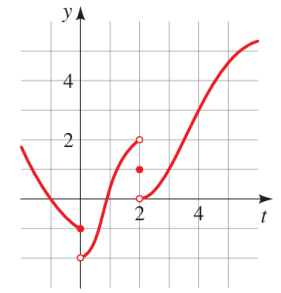
\includegraphics[width=0.4\textwidth]{img/t1-ej3.png}
                \end{figure}
            
                \begin{enumerate}[label=\textbf{\alph*.}]
                    \item \[\bm{\lim_{t \to 0 ^-} g(t)} \approx -1\]
                    \item \[\bm{\lim_{t \to 0 ^+} g(t)} \approx -2\] \newpage
                    \item \[\bm{\lim_{t \to 0} g(t)}\] El límite no existe porque \[\lim_{t \to 0 ^-} g(t) \ne \lim_{t \to 0 ^+} g(t)\]
                    \item \[\bm{\lim_{t \to 2 ^-} g(t)} \approx 2\]
                    \item \[\bm{\lim_{t \to 2 ^+} g(t)} \approx 0\]
                    \item \[\bm{\lim_{t \to 2} g(t)}\] El límite no existe porque \[\lim_{t \to 2 ^-} g(t) \ne \lim_{t \to 2 ^+} g(t)\]
                    \item \[\bm{g(2)} = 1\]
                    \item \[\bm{\lim_{t \to 4} g(t)} \approx 3\]
                \end{enumerate}
            
            % EJERCICIO 4: ---------------------------------------------------
            \vspace{1cm}\hrule
            \item \textbf{Use la tabla de valores para estimar el valor del límite. A continuación, use una calculadora gráfica para confirmar gráficamente sus resultados:}
                \begin{enumerate}[label=\textbf{\arabic*)}] 
                    \item \[\bm{\lim_{x \to -4} \frac{x + 4}{x ^2 + 7x + 12}} \approx -1\]
                        
                        \begin{itemize}
                            \item $\frac{-4.1 + 4}{(-4.1)^2 + 7(-4.1) + 12} =  -0.909$ \hspace{1cm} $\frac{-4.01 + 4}{(-4.01)^2 + 7(-4.01) + 12} =  -0.99$ \vspace{0.2cm} \\$\frac{-4.001 + 4}{(-4.001)^2 + 7(-4.001) + 12} =  -0.999$
                            \item $\frac{-3.999 + 4}{(-3.999)^2 + 7(-3.999) + 12} =  -1.001$ \hspace{1cm} $\frac{-3.99 + 4}{(-3.99)^2 + 7(-3.99) + 12} =  -1.01$ \vspace{0.2cm} \\$\frac{-3.9 + 4}{(-3.9)^2 + 7(-3.9) + 12} =  -1.111$ 
                        \end{itemize}

                        \begin{table}[h]
                            \centering
                            \begin{tabular}{|>{\columncolor{celeste}}l|l|l|l|l|l|l|l|l|l|l|l|}
                                \hline
                                $\bm{x}$    & -4.1 & -4.01 & -4.001  & \textbf{-4} & -3.999 & -3.99 & -3.9 \\
                                \hline
                                $\bm{f(x)}$ & -0.909 & -0.99 & -0.999  & \textit{-1} & -1.001 & -1.01 & -1.111 \\
                                \hline
                            \end{tabular}
                        \end{table}

                        \begin{figure}[h!]
                            \centering
                            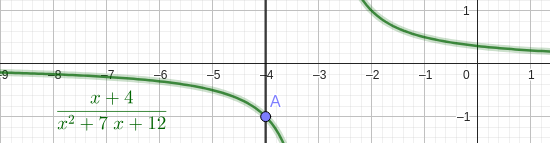
\includegraphics[width=0.7\textwidth]{img/t1-ej4-1.png}
                        \end{figure}
                    
                    

                    \item \[\bm{\lim_{x \to 1} \frac{x ^3 - 1}{x ^2 - 1}} \approx 1.5\]
                    
                        \begin{itemize}
                            \item $\frac{0.9^3 - 1}{0.9^2 - 1} =  1.426 $ \hspace{1cm} $\frac{0.99^3 - 1}{0.99^2 - 1} =  1.493 $ \hspace{1cm}  $\frac{0.999^3 - 1}{0.999^2 - 1} =  1.499 $
                            \item $\frac{1.001^3 - 1}{1.001^2 - 1} =  1.501 $ \hspace{1cm} $\frac{1.01^3 - 1}{1.01^2 - 1} =  1.508 $ \hspace{1cm} $\frac{1.1^3 - 1}{1.1^2 - 1} =  1.576 $
                        \end{itemize}

                        \begin{table}[h]
                            \centering
                            \begin{tabular}{|>{\columncolor{celeste}}l|l|l|l|l|l|l|l|l|l|l|l|}
                                \hline
                                $\bm{x}$    & 0.9 & 0.99 & 0.999  & \textbf{1} & 1.001 & 1.01 & 1.1 \\
                                \hline
                                $\bm{f(x)}$ & 1.426 & 1.493 & 1.499  & \textit{1.5} & 1.501 & 1.508 & 1.576 \\
                                \hline
                            \end{tabular}
                        \end{table}

                        \begin{figure}[h!]
                            \centering
                            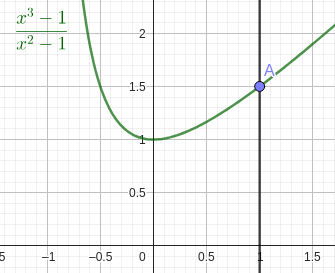
\includegraphics[width=0.4\textwidth]{img/t1-ej4-2.png}
                        \end{figure}
                    
                    
                    \item \[\bm{\lim_{x \to 0} \frac{5 ^x - 3^x }{x}} \approx 0.5\]
                    
                        \begin{itemize}
                            \item $\frac{5^{-0.1} - 3^{-0.1}}{-0.1} = 0.446 $ \hspace{1cm} $\frac{5^{-0.01} - 3^{-0.01}}{-0.01} = 0.504 $ \hspace{1cm} $\frac{5^{-0.001} - 3^{-0.001}}{-0.001} = 0.51 $ 
                            \item $\frac{5^0.001 - 3^0.001}{0.001} =  0.512$ \hspace{1cm} $\frac{5^0.01 - 3^0.01}{0.01} =  0.518$ \hspace{1cm} $\frac{5^0.1 - 3^0.1}{0.1} =  0.585$ \hspace{1cm} 
                        \end{itemize}

                        \begin{table}[h]
                            \centering
                            \begin{tabular}{|>{\columncolor{celeste}}l|l|l|l|l|l|l|l|l|l|l|l|}
                                \hline
                                $\bm{x}$    & -0.1 & -0.01 & -0.001  & \textbf{0} & 0.001 & 0.01 & 0.1 \\
                                \hline
                                $\bm{f(x)}$ & 0.446 & 0.504 & 0.51  & \textit{0.5} & 0.512 & 0.518 & 0.585 \\
                                \hline
                            \end{tabular}
                        \end{table}

                        \newpage
                        \begin{figure}[h!]
                            \centering
                            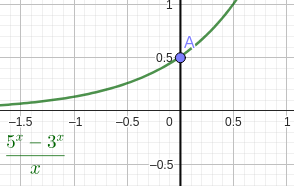
\includegraphics[width=0.4\textwidth]{img/t1-ej4-3.png}
                        \end{figure}
                    
                    
                    \item \[\bm{\lim_{x \to 0} \frac{\sqrt{x + 9} - 3}{x}} \approx 0.17\]
                
                        \begin{itemize}
                            \item $\frac{\sqrt{-0.1 + 9} - 3}{-0.1} = 0.167$ \hspace{1cm} $\frac{\sqrt{-0.01 + 9} - 3}{-0.01} = 0.167$ \hspace{1cm} $\frac{\sqrt{-0.001 + 9} - 3}{-0.001} = 0.167$ 
                            \item $\frac{\sqrt{0.001 + 9} - 3}{0.001} = 0.167$ \hspace{1cm} $\frac{\sqrt{0.01 + 9} - 3}{0.01} = 0.167$ \hspace{1cm} $\frac{\sqrt{0.1 + 9} - 3}{0.1} = 0.166$  
                        \end{itemize}

                        \begin{table}[h]
                            \centering
                            \begin{tabular}{|>{\columncolor{celeste}}l|l|l|l|l|l|l|l|l|l|l|l|}
                                \hline
                                $\bm{x}$    & -0.1 & -0.01 & -0.001  & \textbf{0} & 0.001 & 0.01 & 0.1 \\
                                \hline
                                $\bm{f(x)}$ & 0.167 & 0.167 & 0.167  & \textit{0.17} & 0.167 & 0.167 & 0.166 \\
                                \hline
                            \end{tabular}
                        \end{table}

                        \begin{figure}[h!]
                            \centering
                            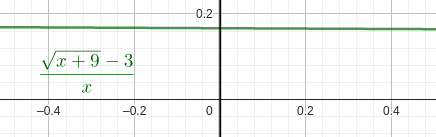
\includegraphics[width=0.7\textwidth]{img/t1-ej4-4.png}
                        \end{figure}
                
                
                \end{enumerate}

            
            % EJERCICIO 5: ---------------------------------------------------
            \vspace{1cm}\hrule
            \item \textbf{Evalúe el límite y justifique cada paso al indicar las leyes de límites apropiadas:}
                \begin{enumerate}[label=\textbf{\arabic*)}] 
                    \item \[\bm{\lim_{x \to 4} (5x ^2 - 2x + 3)}\] Por la ley de la suma/resta: \[\lim_{x \to 4} 5x^2 - \lim_{x \to 4} 2x + \lim_{x \to 4} 3\] Evaluando los límites: \[= 5(4)^2 - 2(4) + 3 = 75\]
                    \item \[\bm{\lim_{x \to 3} (x ^3 + 2)(x ^2 - 5x)}\] Por la ley del producto: \[\lim_{x \to 3} x ^3 + 2 \cdot \lim_{x \to 3} x ^2 - 5x \] Por la ley de la suma/resta: \[\left(\lim_{x \to 3} x^3 + \lim_{x \to 3} 2\right) \cdot \left(\lim_{x \to 3} x^2 - \lim_{x \to 3} 5x\right)\] Evaluando los límites: \[= ((3)^3 + 2) \cdot ((3)^2 - 5(3)) = -174\]
                    \item \[\bm{\lim_{x \to -1} \frac{x - 2 }{x ^2 + 4x - 3}}\] Por la ley del cociente: \[\frac{\lim_{x \to -1} x - 2}{\lim_{x \to -1} x ^2 + 4x - 3}\] Por la ley de la suma/resta: \[\frac{\lim_{x \to -1} x - \lim_{x \to -1}2}{\lim_{x \to -1} x ^2 + \lim_{x \to -1} 4x - \lim_{x \to -1} 3}\] Evaluando los límites: \[= \frac{(-1) - 2}{(-1)^2 + 4(-1) - 3} = 0.5\]
                    \item \[\bm{\lim_{x \to 1} \left(\frac{x^4 + x^2 - 6}{x^4 + 2x + 3}\right)^2}\] Por la ley de la potencia: \[\left(\lim_{x \to 1} \frac{x^4 + x^2 - 6}{x^4 + 2x + 3}\right)^2\] Por la ley del cociente: \[\left(\frac{\lim_{x \to 1} x^4 + x^2 - 6}{\lim_{x \to 1}  x^4 + 2x + 3}\right)^2\] Por la ley de la suma/resta: \[\left(\frac{\lim_{x \to 1} x^4 + \lim_{x \to 1} x^2 - \lim_{x \to 1} 6}{\lim_{x \to 1}  x^4 + \lim_{x \to 1} 2x + \lim_{x \to 1} 3}\right)^2\] Evaluando los límites: \[= \left(\frac{(1)^4 + (1)^2 - 6}{(1)^4 + 2(1) + 3}\right)^2 \approx 0.4444\]
                \end{enumerate}

            
            % EJERCICIO 6: ---------------------------------------------------
            \vspace{1cm}\hrule
            \item \textbf{Evalúe el límite si existe:}
                \begin{enumerate}[label=\textbf{\arabic*)}] 
                    \item \[\bm{\lim_{x \to 2} \frac{x ^2 + x - 6}{x - 2}} = \lim_{x \to 2} \frac{(x + 3)(x - 2)}{x - 2} = \lim_{x \to 2} x + 3 = (2) + 3 = 5\]
                    \item \[\bm{\lim_{x \to -4} \frac{x ^2 + 5x +4}{x ^2 + 3x - 4}} = \lim_{x \to -4} \frac{(x + 4)(x + 1)}{(x + 4)(x - 1)} = \lim_{x \to -4} \frac{x + 1}{x - 1} = \frac{(-4) + 1}{(-4) - 1} = \frac{-3}{-5} = \frac{3}{5}\]
                    \item \[\bm{\lim_{x \to 2} \frac{x ^2 - x + 6}{x + 2}} = \frac{(2)^2 - (2) + 6}{(2) + 2} = \frac{8}{4} = 2\]     
                    \item \[\bm{\lim_{x \to 1} \frac{x ^3 - 1}{x ^2 - 1}} = \lim_{x \to 1} \frac{(x - 1)(x^2 + x + 1)}{(x + 1)(x - 1)} = \lim_{x \to 1} \frac{x^2 + x + 1}{x + 1} = \frac{(1)^2 + (1) + 1}{(1) + 1} = \frac{3}{2}\]
                    \item \[\bm{\lim_{t \to -3} \frac{t ^2 - 9}{2t ^2 + 7t + 3}} = \lim_{t \to -3} \frac{(t - 3)(t + 3)}{(2t + 1)(t + 3)} = \lim_{t \to -3} \frac{t - 3}{2t + 1} = \frac{(-3) - 3}{2(-3) + 1} = \frac{-6}{-5} = \frac{6}{5}\]
                    \item \[\bm{\lim_{h \to 0} \frac{\sqrt{1 + h} - 1}{h}} = \lim_{h \to 0} \frac{\sqrt{1 + h} - 1}{h} \cdot \frac{\sqrt{1 + h} + 1}{\sqrt{1 + h} + 1} = \lim_{h \to 0} \frac{1 + h - 1}{h(\sqrt{1 + h} + 1)}\] \[= \lim_{h \to 0} \frac{1}{\sqrt{1 + h} + 1} = \frac{1}{\sqrt{1 + (0)} + 1} = \frac{1}{2}\] 
                    \item \[\bm{\lim_{h \to 0} \frac{(2 + h) ^3 - 8}{h}} = \lim_{h \to 0} \frac{2^3 + 3(2^2)(h) + 3(2)(h^2) + h^3 - 8}{h}\] \[= \lim_{h \to 0} \frac{12h + 6h^2 + h^3}{h} = \lim_{h \to 0} \frac{h(12 + 6h + h^2)}{h} = \lim_{h \to 0} h^2 + 6h + 12 = (0)^2 + 6(0) + 12 = 12\]
                    \item \[\bm{\lim_{x \to 2} \frac{x ^4 - 16}{x - 2}} = \lim_{x \to 2} \frac{(x^2 + 4)(x^2 - 4)}{x - 2} = \lim_{x \to 2} \frac{(x^2 + 4)(x + 2)(x - 2)}{x - 2}\] \[= \lim_{x \to 2} (x^2 + 4)(x + 2) = ((2)^2 + 4) \cdot ((2) + 2) = 32\]
                    \item \[\bm{\lim_{x \to 7} \frac{\sqrt{x + 2} - 3}{x - 7}} = \lim_{x \to 7} \frac{\sqrt{x + 2} - 3}{x - 7} \cdot \frac{\sqrt{x + 2} + 3}{\sqrt{x + 2} + 3} =  \lim_{x \to 7} \frac{x + 2 - 9}{(x - 7)(\sqrt{x + 2} + 3)}\] \[=  \lim_{x \to 7} \frac{x - 7}{(x - 7)(\sqrt{x + 2} + 3)} = \lim_{x \to 7} \frac{1}{\sqrt{x + 2} + 3} = \frac{1}{\sqrt{(7)+ 2} + 3} = \frac{1}{6}\]
                    \item \[\bm{\lim_{h \to 0} \frac{(3 + h)^{-1} - 3^{-1}}{h}} = \lim_{h \to 0} \frac{(3 + h)^{-1}}{h} - \frac{3^{-1}}{h} = \lim_{h \to 0} \frac{1}{h(3 + h)} - \frac{1}{3h}\] \[= \lim_{h \to 0} \frac{1}{3h + h^2} - \frac{1}{3h} = \lim_{h \to 0} \frac{3h - (3h + h^2)}{(3h + h^2)(3h)} = \lim_{h \to 0} \frac{-h^2}{9h^2 +3h^3} = \lim_{h \to 0} \frac{-h^2}{3h^2(3 + h)}\] \[\lim_{h \to 0} \frac{-1}{9 + 3h} = \frac{-1}{9 + 3(0)} = -\frac{1}{9}\]
                    \item \[\bm{\lim_{x \to -4} \frac{\frac{1}{4} + \frac{1}{x}}{4 + x}} = \lim_{x \to -4} \frac{\frac{x + 4}{4x}}{4 + x} = \lim_{x \to -4} \frac{x + 4}{4x(x + 4)} = \lim_{x \to -4} \frac{1}{4x} = \frac{1}{4(-4)} = -\frac{1}{16}\]
                    \item \[\bm{\lim_{t \to 0} \left(\frac{1}{t} - \frac{1}{t ^2 + t}\right)} = \lim_{t \to 0} \frac{t ^2 + t - t}{t(t ^2 + t)} = \lim_{t \to 0} \frac{t^2}{t^2(t + 1)} = \lim_{t \to 0} \frac{1}{t + 1} = \frac{1}{(0) + 1} = 1\] 
                \end{enumerate}
            
            % EJERCICIO 7: ---------------------------------------------------
            \vspace{1cm}\hrule
            \item \textbf{Encuentre el límite, si existe. Si el límite no existe, explique por qué:}
                \begin{enumerate}[label=\textbf{\arabic*)}] 
                    \item \[\bm{\lim_{x \to -4} \left| x + 4 \right|}\]
                    \item \[\bm{\lim_{x \to -4 ^-} \frac{\left| x + 4 \right|}{x + 4}}\]
                    \item \[\bm{\lim_{x \to 2} \frac{\left| x - 2 \right|}{x - 2}}\]
                    \item \[\bm{\lim_{x \to 1.5} \frac{2x ^2 - 3x}{\left| 2x - 3 \right|}}\]
                    \item \[\bm{\lim_{x \to 0 ^-} \left(\frac{1}{x} - \frac{1}{\left| x \right|}\right)}\]
                    \item \[\bm{\lim_{x \to 0 ^+} \left(\frac{1}{x} - \frac{1}{\left| x \right|}\right)}\]
                \end{enumerate}


            % EJERCICIO 8: ---------------------------------------------------
            \vspace{1cm}\hrule
            \item \textbf{Sea: }
                \[
                    \boldsymbol{
                        f(x) = 
                        \left\{
                            \begin{array}{ll}
                                x - 1 & ,\ \text{si} \ x < 2 \\
                                x ^2 - 4x + 6 & ,\ \text{si} \ x \geq 2
                            \end{array}
                        \right.
                    }
                \]

            % EJERCICIO 9: ---------------------------------------------------
            \vspace{1cm}\hrule
            \item \textbf{Sea: }
                \[
                    \boldsymbol{
                        h(x) = 
                        \left\{
                            \begin{array}{ll}
                                x & ,\ \text{si} \ x < 0 \\
                                x ^2 & ,\ \text{si} \ 0 < x \leq 2 \\
                                8 - x & ,\ \text{si} \ x > 2
                            \end{array}
                        \right.
                    }
                \]
            
            
            % EJERCICIO 10: ---------------------------------------------------
            \vspace{1cm}\hrule
            \item \textbf{Resuelva los siguientes límites al infinito:}
                \begin{enumerate}[label=\textbf{\arabic*)}] 
                    \item \[\bm{\lim_{x \to +\infty} \left( \frac{x^3 + 1}{x - 1} - \frac{x}{4} \right)}\]
                    \item \[\bm{\lim_{x \to +\infty} \left( 4x^2 - \sqrt{x^4 + 1} \right)}\]
                    \item \[\bm{\lim_{x \to +\infty} \left( 2x - 1 - \sqrt{4x^2 + 1} \right)}\]
                    \item \[\bm{\lim_{x \to +\infty} \frac{5x + 8}{-5x + 2}}\]
                    \item \[\bm{\lim_{x \to -\infty} \frac{x^2 + 3x + 5}{x^4 - x - 6}}\]
                    \item \[\bm{\lim_{x \to +\infty} \frac{\sqrt[3]{x^7 - 4x^3}}{x^2 + 5x}}\]
                \end{enumerate}

        
        \end{enumerate}

\end{document}